%% ----------------------------------------------------------------
%% Thesis.tex -- main
%% ---------------------------------------------------------------- 

\documentclass[a4paper, 10pt, oneside]{memoir}
%% Use the option citeauthor to be able to use citet. The default cite will still work.
\usepackage[citeauthor]{basilea}

%% ----------------------------------------------------------------

\title				{Thesis Title}
\thesistype			{Bachelor thesis}

\department 		    {Department of Mathematics and Computer Science}
\faculty			{Natural Science Faculty of the University of Basel}
\research		    {Artificial Intelligence \\ https://ai.dmi.unibas.ch/}

\examiner    		{Prof. Dr. Malte Helmert}
\supervisor  		{Dr. Travis Rivera Petit and Dr. David Speck}

\authors     		{Pascal von Fellenberg}
\email				{pascal.vonfellenberg@unibas.ch}
\immatriculnr		{}

\date				{\today}

% switch here for the german logo to logo-de
\ulogo				{Template/logo-en} 


%% ----------------------------------------------------------------
\begin{document}

% for english use \selectlanguage{english}, for german use \selectlanguage{ngerman}
\selectlanguage{english}

\thesisfront
\maketitle
\pagestyle{thesis}
%% ----------------------------------------------------------------
% % !TEX root = ../Thesis.tex
\chapter{Acknowledgments}
TODO

%% ----------------------------------------------------------------
% !TEX root = ../Thesis.tex
\chapter{Abstract}
TODO
%% ----------------------------------------------------------------
\thesistoc
%% ----------------------------------------------------------------
%\thesisnomencl
%% ----------------------------------------------------------------
\thesismain
\chapter{Background}

In this chapter, we cover some Definitions relevant for this thesis.

\section{Deterministic Finite Automaton}
\textbf{Definition:} A deterministic finite automaton (DFA) is a 5-tuple $M = \langle Q, \Sigma, \delta, q_0, F \rangle$ where
\begin{itemize}
    \item $Q$ is the finite set of states
    \item $\Sigma$ is the input alphabet
    \item $\delta : Q \times \Sigma \rightarrow Q$ is the transition function
    \item $q_0 \in Q$ is the start state
    \item $F \subseteq Q$ is the set of accept states (or final states).
\end{itemize}

\textbf{Definition:} DFA $M = \langle Q, \Sigma, \delta, q_0, F \rangle$ accepts the word $w = a_1 \ldots a_n$ if there is a sequence of states $q'_0, \ldots, q'_n \in Q$ with
\begin{itemize}
    \item $q'_0 = q_0$
    \item $\delta(q'_{i-1}, a_i) = q'_i$ for all $i \in \{1, \ldots, n\}$ and
    \item $q'_n \in F$.
\end{itemize}

\textbf{Definition:} Let $M$ be a DFA. The language recognized by $M$ is defined as $\mathcal L(M) = \{w \in \Sigma^* \mid w \text{ is accepted by } M\}$.

We depict a DFA visually as a directed graph with labelled arcs, where there is a corresponding node for each state and a labelled arc for each transition in the transition function.


%% ----------------------------------------------------------------
\thesisappendix
\thesisbib
\begin{appendices}
	% !TEX root = ../Thesis.tex
\chapter{Appendix}
\end{appendices}
%% ----------------------------------------------------------------
\thesisback
\iflanguage{english}
  {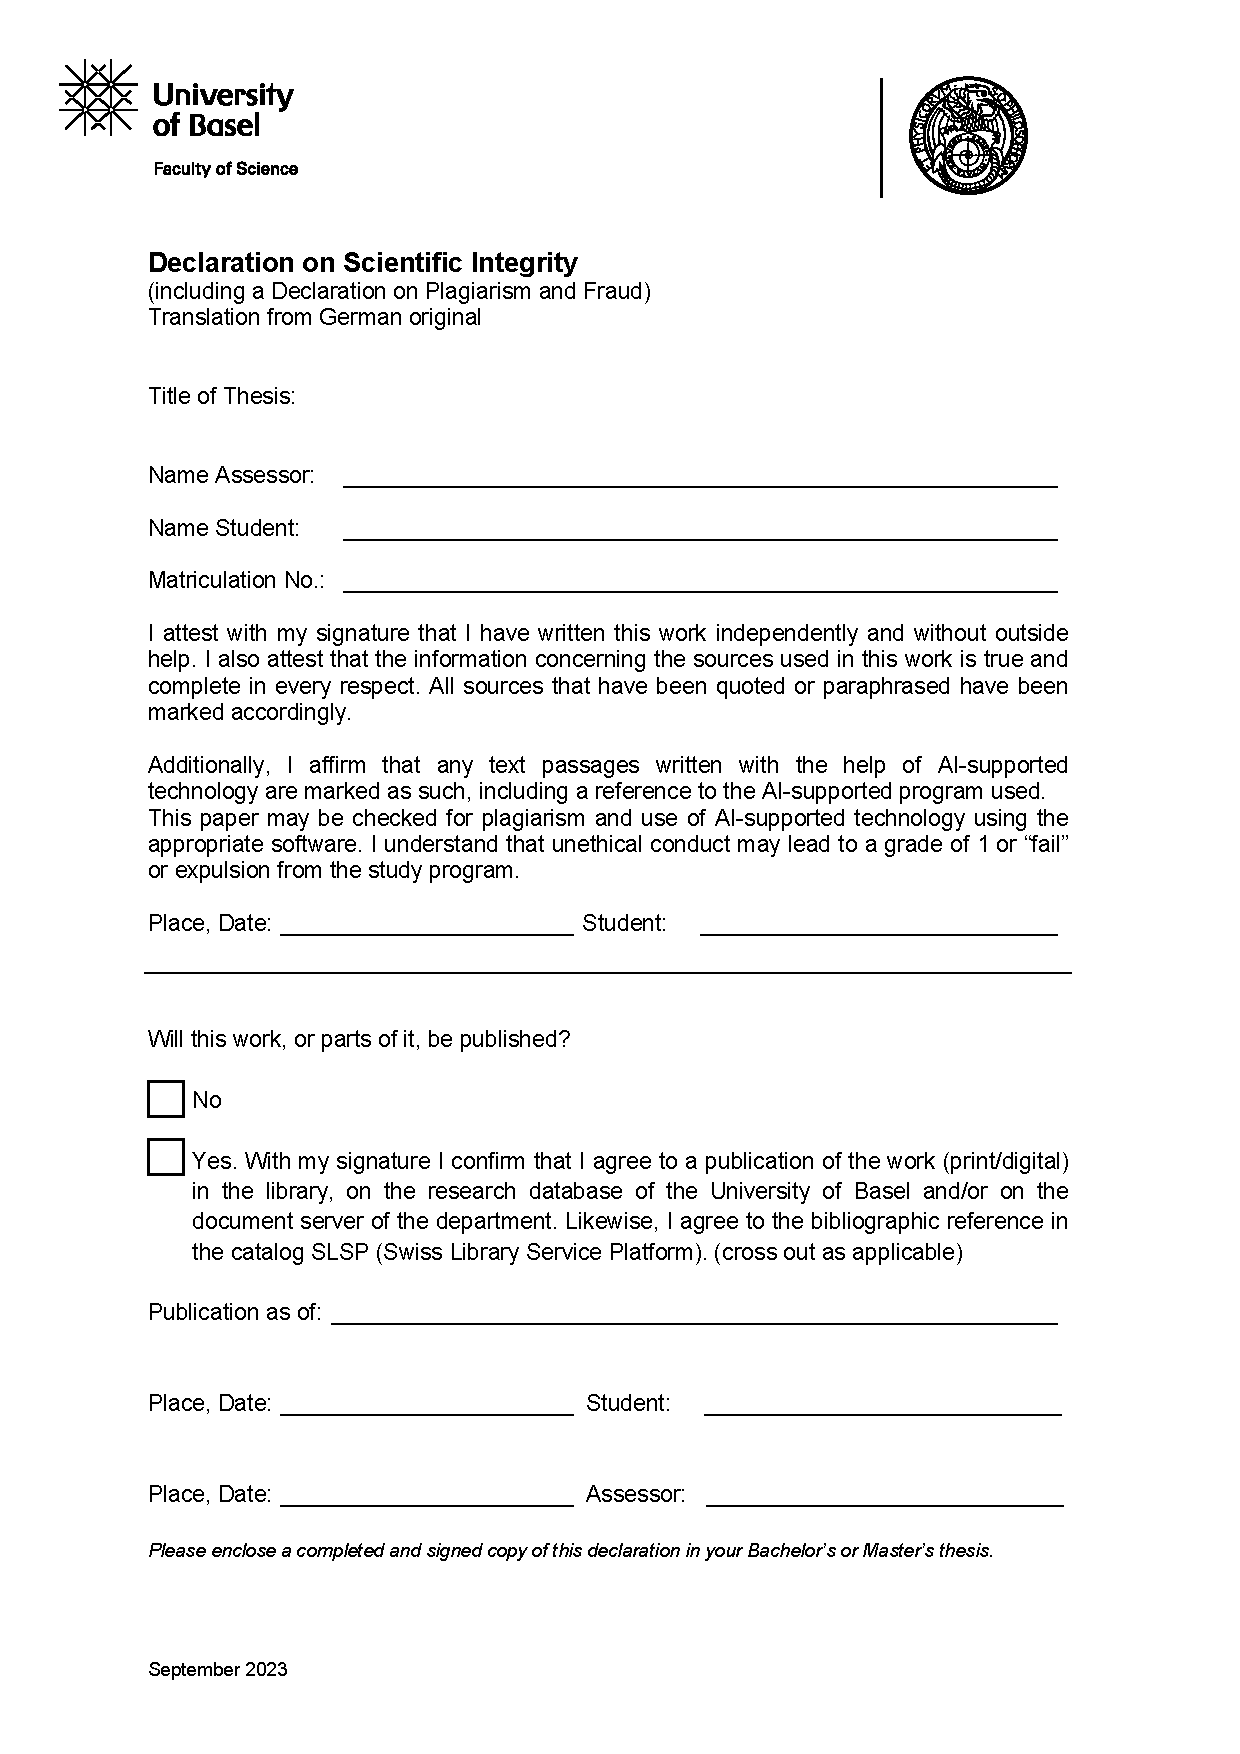
\includepdf{./Back/wissensch_Redlichkeit_E_09-2023.pdf}}
  {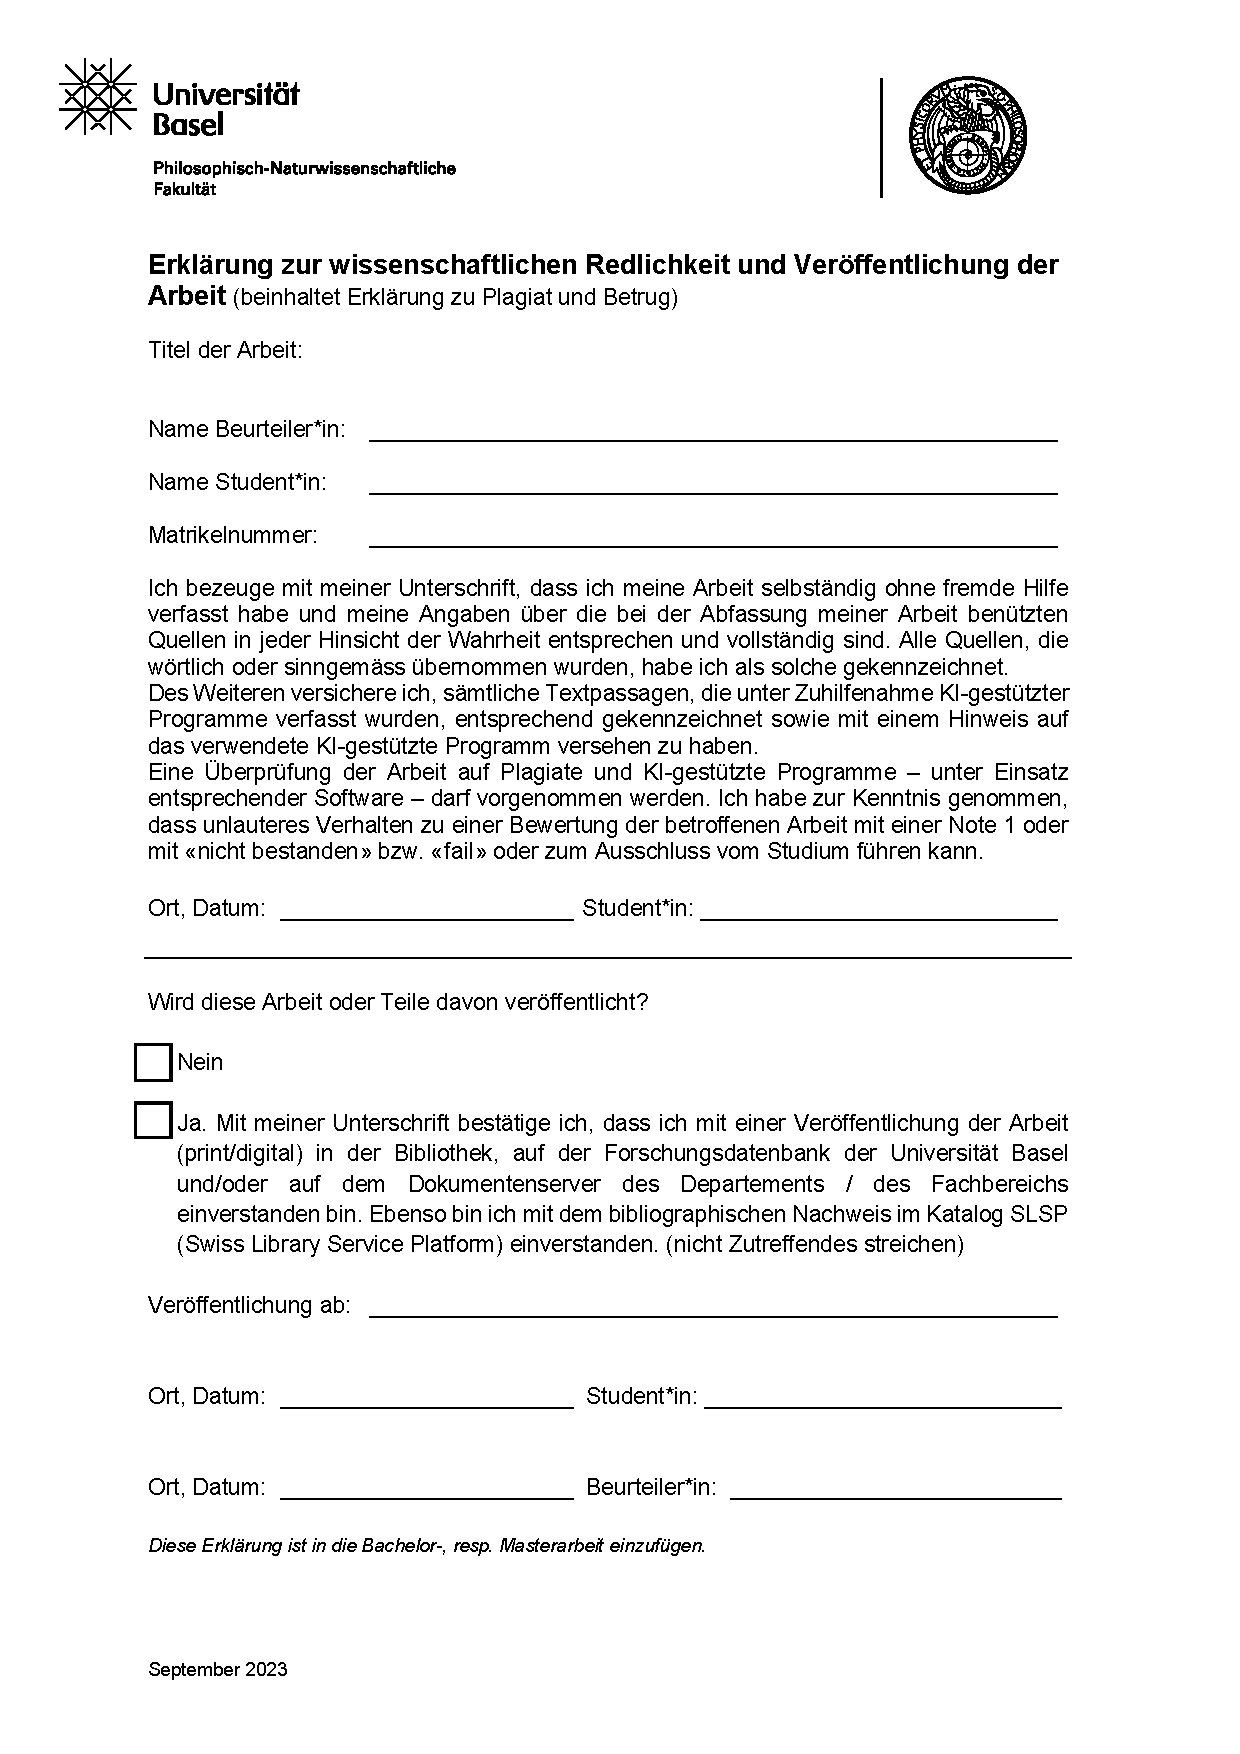
\includepdf{./Back/wissensch_Redlichkeit_D_09-2023.pdf}}
%% ----------------------------------------------------------------
\end{document}
%% ----------------------------------------------------------------
